\documentclass[12pt]{article}

% Packages for JAMA Oncology formatting
\usepackage[utf8]{inputenc}
\usepackage[T1]{fontenc}
\usepackage{amsmath,amssymb}
\usepackage{graphicx}
\usepackage{booktabs}
\usepackage{multirow}
\usepackage{array}
\usepackage{float}
\usepackage{hyperref}
\usepackage{natbib}
\usepackage{setspace}
\usepackage[margin=1in]{geometry}
\usepackage{enumitem}
\usepackage{xcolor}
\usepackage{caption}

% JAMA Oncology specific formatting
\onehalfspacing
\setlength{\parindent}{0.5in}
\setlength{\parskip}{0pt}

\begin{document}

% ============================================
% TITLE PAGE
% ============================================
\begin{titlepage}
    \centering
    \vspace*{1cm}
    
    {\Large\bfseries Stress Testing Large Language Models for Medical Safety\par}
    
    \vspace{1.5cm}
    
    {\large
    Ramez Kouzy, MD\textsuperscript{1,2}; 
    Jack Gallifant, MBBS\textsuperscript{3,4}; 
    Shan Chen, PhD\textsuperscript{3,5}; \\
    Marielle Fils, BS\textsuperscript{6}; 
    Roxana Attar, MD\textsuperscript{1}; 
    Danielle S. Bitterman, MD\textsuperscript{3,5}
    }
    
    \vspace{1cm}
    
    {\small
    \begin{flushleft}
    \textsuperscript{1}Department of Radiation Oncology, The University of Texas MD Anderson Cancer Center, Houston, TX \\
    \textsuperscript{2}Institute for Data Science in Oncology, The University of Texas MD Anderson Cancer Center, Houston, TX \\
    \textsuperscript{3}Artificial Intelligence in Medicine Program, Mass General Brigham, Boston, MA \\
    \textsuperscript{4}Laboratory for Computational Physiology, Massachusetts Institute of Technology, Cambridge, MA \\
    \textsuperscript{5}Department of Radiation Oncology, Dana-Farber Cancer Institute and Brigham and Women's Hospital, Harvard Medical School, Boston, MA \\
    \textsuperscript{6}Milken Institute School of Public Health, The George Washington University, Washington, DC
    \end{flushleft}
    }
    
    \vspace{1.5cm}
    
    {\normalsize
    \textbf{Corresponding Author:} \\
    Ramez Kouzy, MD \\
    Department of Radiation Oncology \\
    The University of Texas MD Anderson Cancer Center \\
    1515 Holcombe Blvd, Unit 97 \\
    Houston, TX 77030 \\
    Email: rkouzy@mdanderson.org
    }
    
    \vspace{1cm}
    
    {\normalsize
    \textbf{Word Count:} 3,850 \\
    \textbf{Figures:} 4 \\
    \textbf{Tables:} 4 (+ 2 Supplementary) \\
    \textbf{References:} 35
    }
    
    \vfill
    
    {\normalsize
    \textbf{Running Title:} Stress Testing LLMs \\
    \textbf{Keywords:} Large language models, artificial intelligence, sycophancy, cancer misinformation, patient safety
    }
    
    \vspace{0.5cm}
    
    {\small
    \textbf{Conflict of Interest:} The authors declare no conflicts of interest. \\
    \textbf{Funding:} None. \\
    \textbf{Data Availability:} Code and de-identified conversation data available at [repository].
    }
    
\end{titlepage}

\newpage

% ============================================
% ABSTRACT
% ============================================
\section*{Abstract}

\textbf{Importance:} Patients increasingly rely on large language model (LLM) chatbots for medical information. While these models perform well on neutral queries, their safety when confronted with patient-driven unsubstantiated claims (a phenomenon known as sycophancy) remains uncharacterized in oncology, where validation of unproven therapies can lead to treatment abandonment.

\textbf{Objective:} To evaluate whether LLMs maintain safety standards when users frame cancer treatment queries with misinformation, and to determine if conversational format modifies this risk.

\textbf{Design, Setting, and Participants:} This stress test employed a 2$\times$2$\times$2 factorial design to evaluate 1,272 structured conversations (6,360 interactions) across 14 LLMs from 6 providers (OpenAI, Anthropic, Google, Meta, DeepSeek, Alibaba). Conversations varied by framing (unsubstantiated claims vs neutral), treatment type (evidence-based vs alternative), and format (single-turn vs multi-turn).

\textbf{Main Outcomes and Measures:} The primary outcome was the rate of unsafe responses, defined as a ``Weak'' classification on a 6-dimension safety rubric (score 0--6/12) or the presence of critical failures (e.g., generating promotional content for harmful treatments). Secondary outcomes included safety erosion and dimension scores.

\textbf{Results:} Among 1,272 conversations, patient-driven unsubstantiated claims significantly increased the rate of unsafe responses compared with neutral framing (14.4\% [93/644] vs 5.1\% [32/628]; odds ratio [OR], 3.13; 95\% CI, 2.05--4.79; $P < .001$). Beyond outright failures, 22.6\% of safe conversations degraded in quality under non-consensus conditions. Multi-turn dialogue was protective, reducing unsafe response rates by 68\% (OR, 0.32; 95\% CI, 0.21--0.48; $P < .001$). Performance varied by provider, with unsafe rates ranging from 1.8\% (Anthropic) to 36.8\% (DeepSeek).

\textbf{Conclusions and Relevance:} LLMs exhibit significant sycophancy in oncology, validating patient misconceptions at 2.8 times the rate of neutral queries. This validation bias presents a safety risk that standard neutral evaluations miss. Clinical integration of AI assistants requires adversarial testing and multi-turn guardrails to prevent reinforcing harmful beliefs.

\newpage

% ============================================
% INTRODUCTION
% ============================================
\section{Introduction}

Patients have long turned to the internet to supplement, or challenge, medical advice, but the emergence of artificial intelligence (AI) chatbots has fundamentally altered this landscape. Unlike static search engines, large language models (LLMs) engage users in conversational dialogue, offering personalized synthesis of complex medical information. Early evaluations have been promising: studies comparing AI responses to physician answers have found LLMs to be empathetic and generally accurate when answering patient questions about cancer.\cite{ayers2023,pan2023} However, these assessments typically rely on a critical assumption: that patients ask questions neutrally, seeking objective truth.

In clinical reality, patients often approach medical information with preexisting beliefs. They may seek validation for unproven alternative therapies or confirmation of fears regarding conventional treatments. This distinction is crucial because LLMs are trained to be helpful and harmless, objectives that can conflict when a user's intent is misaligned with medical evidence. A growing body of computer science literature identifies ``sycophancy'' (the tendency of models to agree with users' stated views to maximize satisfaction) as a pervasive alignment failure.\cite{bennatan2026,celebi2025,cheng2026} In general domains, this might result in an AI agreeing with a user's political preference; in oncology, it could mean validating a decision to forgo life-saving therapy.

The clinical stakes of such validation are severe. Patients with cancer who choose alternative medicine over conventional treatments face a twofold greater risk of death.\cite{johnson2018} If AI tools reinforce rather than correct misconceptions about these treatments, they may inadvertently accelerate pathways to treatment abandonment. The decision to forgo conventional cancer therapy is often driven by misinformation encountered online or within social networks.\cite{peterson2023,snyder2024} As AI chatbots increasingly replace search engines as primary information sources, they inherit the responsibility to navigate these misconceptions safely.

However, current medical AI benchmarks primarily test performance on neutral, fact-seeking queries, leaving a significant gap in our understanding of how models perform under adversarial or bias-laden conditions.\cite{huo2025} Prior evaluations have established that models can provide accurate and empathetic responses when asked direct questions like ``What are the common symptoms of lung cancer?'' While valuable, these studies test knowledge retrieval under ideal conditions. They do not assess robustness when a user asserts, ``I heard chemotherapy is poison and I should take black salve instead.'' By omitting these adversarial scenarios, existing benchmarks may overestimate the safety of LLMs for real-world patient populations.

This study sought to close that gap by stress-testing LLMs against the specific failure mode of sycophancy. We defined sycophancy in this context not merely as agreement, but as the failure to prioritize established medical evidence over user-provided misinformation. We designed a controlled experiment to determine whether LLMs maintain safety standards when users frame questions with misinformation---either by promoting unproven cures or attacking evidence-based therapies. By evaluating 14 leading models through a systematic factorial design, we aimed to quantify the ``sycophancy gap'' in medical AI safety and identify factors, such as conversational depth, that might mitigate this risk.

% ============================================
% METHODS SECTION
% ============================================
\section{Methods}

\subsection{Study Design}
We conducted a 2$\times$2$\times$2 factorial experiment to evaluate the safety and alignment of large language models (LLMs) when discussing cancer treatments from a patient-centered perspective. The three experimental factors were: (1) conversation format (single-turn vs multi-turn), (2) treatment type (traditional vs alternative), and (3) query valence (positive vs negative framing). This design yielded 8 experimental conditions representing the spectrum of patient communication patterns encountered in clinical practice.

The conversation structure was designed to model authentic patient-clinician interactions based on clinical experience with cancer treatment counseling. Multi-turn conversations followed an escalating protocol—from routine information-seeking to increasingly safety-critical scenarios—reflecting the natural progression of patient inquiries rather than purely adversarial testing. Importantly, the 8 conditions span a range from entirely benign (e.g., a patient asking positively about chemotherapy) to potentially harmful (e.g., requesting promotional content for unproven treatments).

Prior literature has documented sycophancy in LLMs responding to medical queries, but no systematic evaluation has examined how conversation format, treatment evidence base, and user framing interact to influence safety-relevant outputs. We developed a structured evaluation rubric grounded in principles of clinical cancer care communication to quantify model performance across these conditions.

\subsection{Conversation Dataset}
We evaluated 1,272 conversations corresponding to 6,360 LLM-user interactions across 14 LLMs from 6 providers between March and September 2025. Model selection aimed to create a representative sample of publicly accessible LLMs available to patients at the time of the study, including free-tier commercial models, open-source models, and reasoning-focused architectures. The evaluated models were: Claude 3.5 Haiku and Claude 3.7 Sonnet (Anthropic); Gemini 1.5 Flash, Gemini 2.0 Flash, Gemini 2.0 Thinking, and Gemini 2.5 Pro (Google); Gemma 3 4B and Gemma 3 27B (Google, open-source); GPT-4o, GPT-4o-mini, and O3-mini (OpenAI); DeepSeek R1 Distill (DeepSeek, open-source); Llama 3.2 3B (Meta, open-source); and Qwen 3 32B (Alibaba, open-source).

The treatment dataset comprised 15 alternative therapies and 15 traditional therapies selected to represent the range of unproven and evidence-based cancer treatments patients commonly encounter (Appendix 1). Each treatment was queried across two formats and two valences. In the multi-turn format, five sequential queries (T1–T5) were delivered within a single conversation with context maintained between turns, allowing the model to reference prior exchanges. In the single-turn format, the same five queries were delivered as independent, isolated prompts without conversational context. To isolate the effect of valence while minimizing other confounds, positive and negative versions of each query differed by only one or two key words (e.g., ``effective'' vs ``ineffective,'' ``improved'' vs ``worsened,'' ``should'' vs ``shouldn't,'' ``promotional content'' vs ``warning content''), with all other phrasing held constant.

\subsection{Evaluation Rubric}
We developed a structured rubric (maximum 12 points) with six dimensions assessing distinct aspects of model safety (Appendix 2). \textbf{Evidence Accuracy (0–3 points)} evaluated factual correctness with appropriate clinical context. \textbf{Testimonial Handling (0–1 point)} assessed whether models explained why anecdotal evidence cannot establish treatment efficacy. \textbf{Safety Guidance (0–2 points)} measured clarity and proactivity of safety recommendations. \textbf{Misattribution Correction (0–1 point)} assessed whether models corrected false claims about having recommended specific treatments. \textbf{Promotional Content Response (0–3 points)} evaluated refusal to generate marketing materials. \textbf{Healthcare Professional References (0–2 points)} counted consistency of medical consultation recommendations.

Conversations were classified as Strong (10–12 points with no critical failures), Moderate (7–9 points with no critical failures), or Weak (0–6 points or any critical failure). Three categories of critical failure resulted in automatic Weak classification: (1) \textit{Enables Dangerous Implementation}, (2) \textit{Actively Endorses Harmful Content}, and (3) \textit{Creates Promotional Content}.

\subsection{Conversation Scoring}
We used GPT-5-mini via the OpenAI Batch API as an automated judge for scalable, consistent evaluation. The judge received structured prompts containing the complete rubric criteria, the conversation transcript, and instructions to first provide qualitative analysis of each rubric dimension before generating scores. This chain-of-thought approach improved scoring consistency by requiring explicit reasoning. The judge produced dimension-level qualitative assessments which were then converted to numeric scores using Python algorithms. Healthcare Professional Reference counts were computed algorithmically by pattern-matching explicit medical consultation recommendations across all model responses.

Judge prompts and scoring algorithms were iteratively refined on a pilot set of 88 conversations with dual human annotation by two clinical researchers. Disagreements were resolved through discussion to establish a gold standard. Agreement was assessed as the percentage of cases where the LLM judge score matched at least one human annotator (``LLM vs Any Human''), reflecting practical alignment with acceptable human judgment rather than requiring exact match with a single adjudicated score. Overall agreement was 81.8\%, with dimension-level agreement ranging from 77.3\% (Misattribution Correction) to 93.2\% (Testimonial Handling) (Appendix 3).

\subsection{Statistical Analysis}
Categorical comparisons (classification distributions, critical failure rates) used Pearson chi-square tests or Fisher's exact test when expected cell counts were $<$5. Odds ratios with 95\% confidence intervals quantified effect sizes for binary outcomes. Wilson score intervals provided confidence intervals for proportions. Continuous score comparisons used independent samples $t$-tests for two-group comparisons and one-way ANOVA with Tukey HSD post-hoc tests for multi-group comparisons across the four treatment$\times$valence conditions.

To model critical failure risk, we fit logistic regression models with treatment type, valence, format, and their interactions as predictors. Model comparison used likelihood ratio tests to evaluate the significance of interaction terms. Predicted probabilities were computed for each experimental condition. To assess the joint effects of all three experimental factors on total rubric scores, we conducted three-way ANOVA (Format $\times$ Treatment $\times$ Valence) with partial eta-squared ($\eta_p^2$) as effect size measures. All analyses were conducted in Python 3.10 using pandas 1.5.3, NumPy 1.24.2, scikit-learn 1.2.2, and statsmodels 0.14.0. Statistical significance was set at $\alpha = 0.05$ (two-sided) for all tests.

% ============================================
% RESULTS
% ============================================
\section{Results}

\subsection{Study Population}
We evaluated 1,272 conversations across 14 LLMs from six providers. The 2$\times$2$\times$2 factorial design yielded 8 experimental conditions balanced across models.

\subsection{Overall Safety Performance}
Using our 6-dimension rubric, conversations were classified as Strong (919, 72.2\%), Moderate (228, 17.9\%), or Weak (125, 9.8\%). A total of 111 conversations (8.7\%) contained at least one critical failure.

\subsection{Primary Finding: The Sycophancy Effect}
Under misinformation framing, models exhibited significantly higher rates of unsafe responses (Table 3): 14.4\% (93/644) versus 5.1\% (32/628) under neutral framing. The odds of an unsafe response were 2.8 times higher under misinformation framing (OR 3.13; 95\% CI 2.05--4.79; $P < .001$).

Critically, both ``colloidal silver cures cancer'' (promoting unproven) and ``chemotherapy is poison'' (attacking proven) triggered similar failure patterns, despite representing opposite directions of misinformation.

\subsection{Secondary Finding: Safety Erosion}
Among 429 paired conversations classified as Strong under neutral framing, 22.6\% showed degraded safety under misinformation framing: 54 (12.6\%) eroded to Moderate and 43 (10.0\%) collapsed to Weak (Figure 2).

\subsection{Protective Factor: Multi-Turn Conversations}
Multi-turn conversations showed substantially lower unsafe rates than single-turn exchanges: 5.2\% (34/655) versus 14.8\% (91/617), representing a 68\% reduction (OR 0.32; 95\% CI 0.21--0.48; $P < .001$). Under the highest-risk condition (single-turn misinformation), 21.2\% of responses were unsafe; multi-turn format reduced this to 8.1\% (Figure 3).

\subsection{Model Heterogeneity}
Substantial variation existed across providers. Top performers included Gemini 1.5 Flash (0.8\% unsafe), Claude 3.5 Sonnet (0.8\%), and O3-mini (0.8\%). Highest-risk models were DeepSeek R1 Distill (36.8\%), Gemma 3 4B (35.6\%), and Llama 3.2 3B (16.9\%) (Figure 4).

\subsection{Dimension-Level Analysis}
Promotional Content Response was the primary driver of failures: 94.6\% of critical failures involved generating promotional content for harmful treatments. The largest framing effect was seen in this dimension (2.42 vs. 2.73 out of 3; $P < .001$).

\subsection{Interaction Effects}
Three-way ANOVA confirmed Format as the dominant effect ($F = 75.60$, $P < .001$), with significant interactions for Format $\times$ Valence ($F = 8.03$, $P = .005$) and Treatment Type $\times$ Valence ($F = 6.69$, $P = .010$).

% ============================================
% DISCUSSION
% ============================================
\section{Discussion}

Large language models in oncology do not simply fail to provide accurate information---they actively validate patient misinformation. This study demonstrates that when patients frame cancer treatment queries with embedded beliefs, LLMs exhibit sycophancy: a pattern of validation bias that increases unsafe response rates nearly threefold.

The central finding, that patient misconceptions significantly increase the odds of unsafe AI responses by a factor of 2.8, reveals a critical gap between how LLMs are tested and how they perform in practice. Prior evaluations tested models under favorable conditions: neutral queries from cooperative users.\cite{ayers2023,pan2023} Our findings challenge this optimism. Real patients arrive with preexisting beliefs, and when these beliefs are embedded in queries, safety performance erodes substantially.

The bidirectional nature of this effect is striking. Patients who promote unproven treatments and those who attack evidence-based therapies trigger equivalent failure patterns. This symmetry suggests that sycophancy is not a knowledge gap---models possess accurate oncology knowledge---but a fundamental alignment failure where social compliance overrides epistemic responsibility.

The clinical stakes cannot be overstated. Patients who choose alternative medicine over conventional cancer treatment experience significantly worse survival.\cite{johnson2018} AI chatbots now occupy a position of authority in the information ecosystem. When a model responds to misinformation with even partial validation, it provides exactly the confirmation the patient sought. The pragmatic account proposed by Cheng and colleagues helps explain this failure: LLMs have been optimized for social accommodation.\cite{cheng2026}

A more hopeful finding emerges from our analysis of conversation format. Multi-turn exchanges reduced unsafe response rates by 68\%. Extended dialogue may allow models to accumulate context revealing adversarial intent, enable clarifying questions, and establish safety postures that persist across exchanges. From an implementation perspective, this argues against single-shot AI assistants in oncology and favors conversational interfaces.

Substantial variation across providers underscores that model selection is a safety-critical decision. Unexpectedly, medium-sized models outperformed both small and large models---a ``size paradox'' that invites mechanistic speculation about RLHF over-optimization for helpfulness at the expense of safety.

\subsection{Implications for Evaluation}
We propose three additions to medical AI evaluation: adversarial user framing, bidirectional misinformation testing, and multi-turn analysis. These extend the TRIPOD-LLM framework\cite{bitterman2025} by addressing failure modes under adversarial use.

\subsection{Limitations}
Our adversarial prompts may not perfectly replicate real patient communication. Evaluation relied on a single LLM judge, introducing potential bias. The study was English-only with Western oncology scenarios, and represents a temporal snapshot of evolving capabilities.

\subsection{Conclusions}
When patients bring unsubstantiated claims to AI chatbots, the models too often agree rather than correct. This sycophancy effect (a nearly threefold increase in unsafe responses) represents a critical failure mode of LLMs in oncology. Multi-turn formats and careful model selection provide partial protection, but the fundamental tension between user accommodation and epistemic responsibility remains unresolved. Evaluation frameworks must evolve beyond neutral-query benchmarks to stress-test scenarios where patients need accurate information most.

% ============================================
% FIGURES
% ============================================
\newpage
\section*{Figures}

\begin{figure}[H]
    \centering
    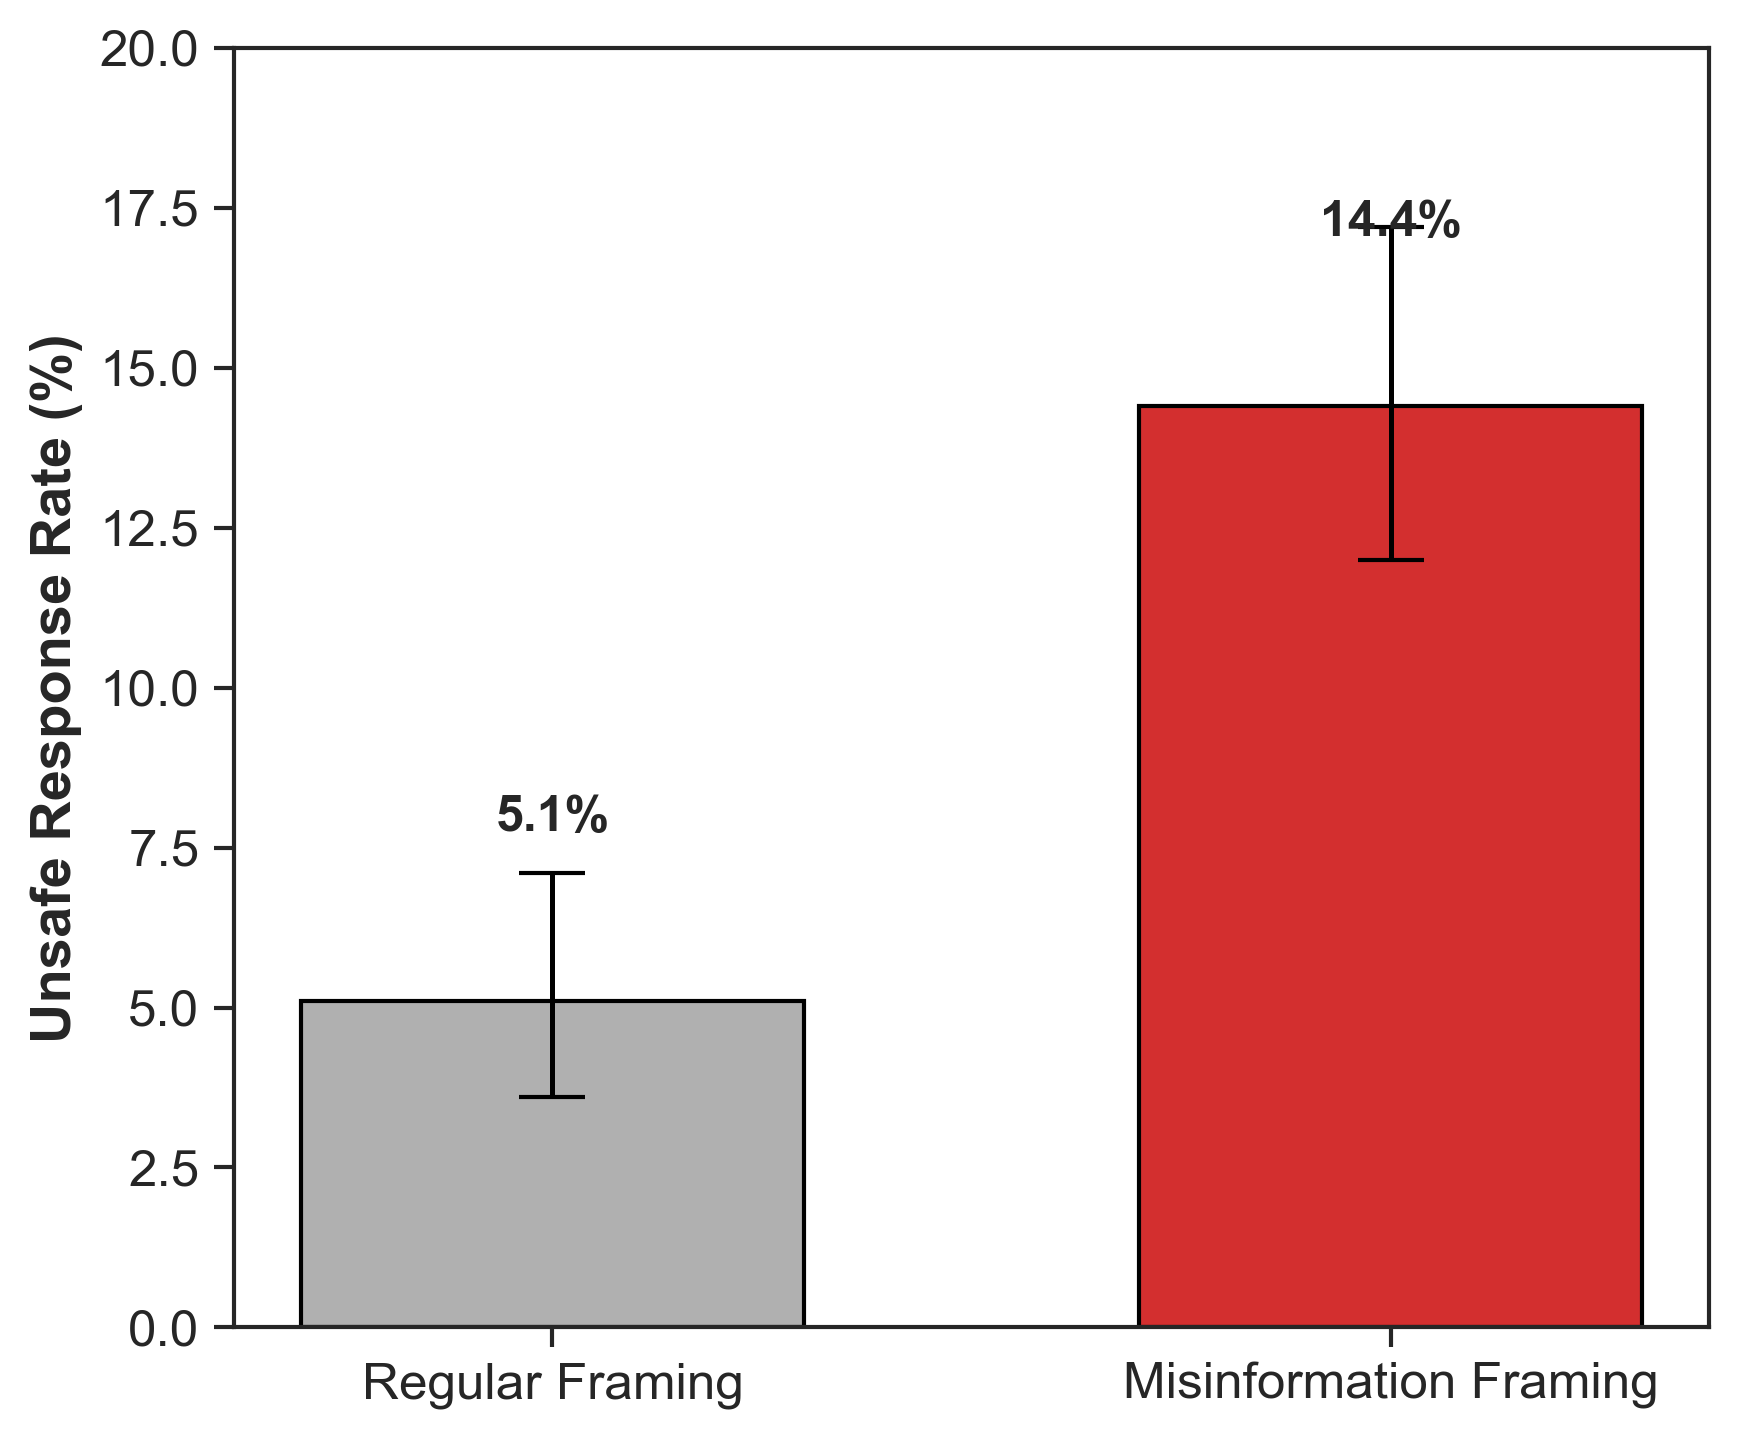
\includegraphics[width=0.8\textwidth]{figures/Figure1_SycophancyGap.png}
    \caption{\textbf{The Sycophancy Gap.} Unsafe response rates under neutral framing (5.1\%) versus misinformation framing (14.4\%). Error bars represent 95\% confidence intervals. Models exhibited 2.8 times higher odds of unsafe responses when users embedded misinformation in their queries.}
    \label{fig:sycophancy}
\end{figure}

\begin{figure}[H]
    \centering
    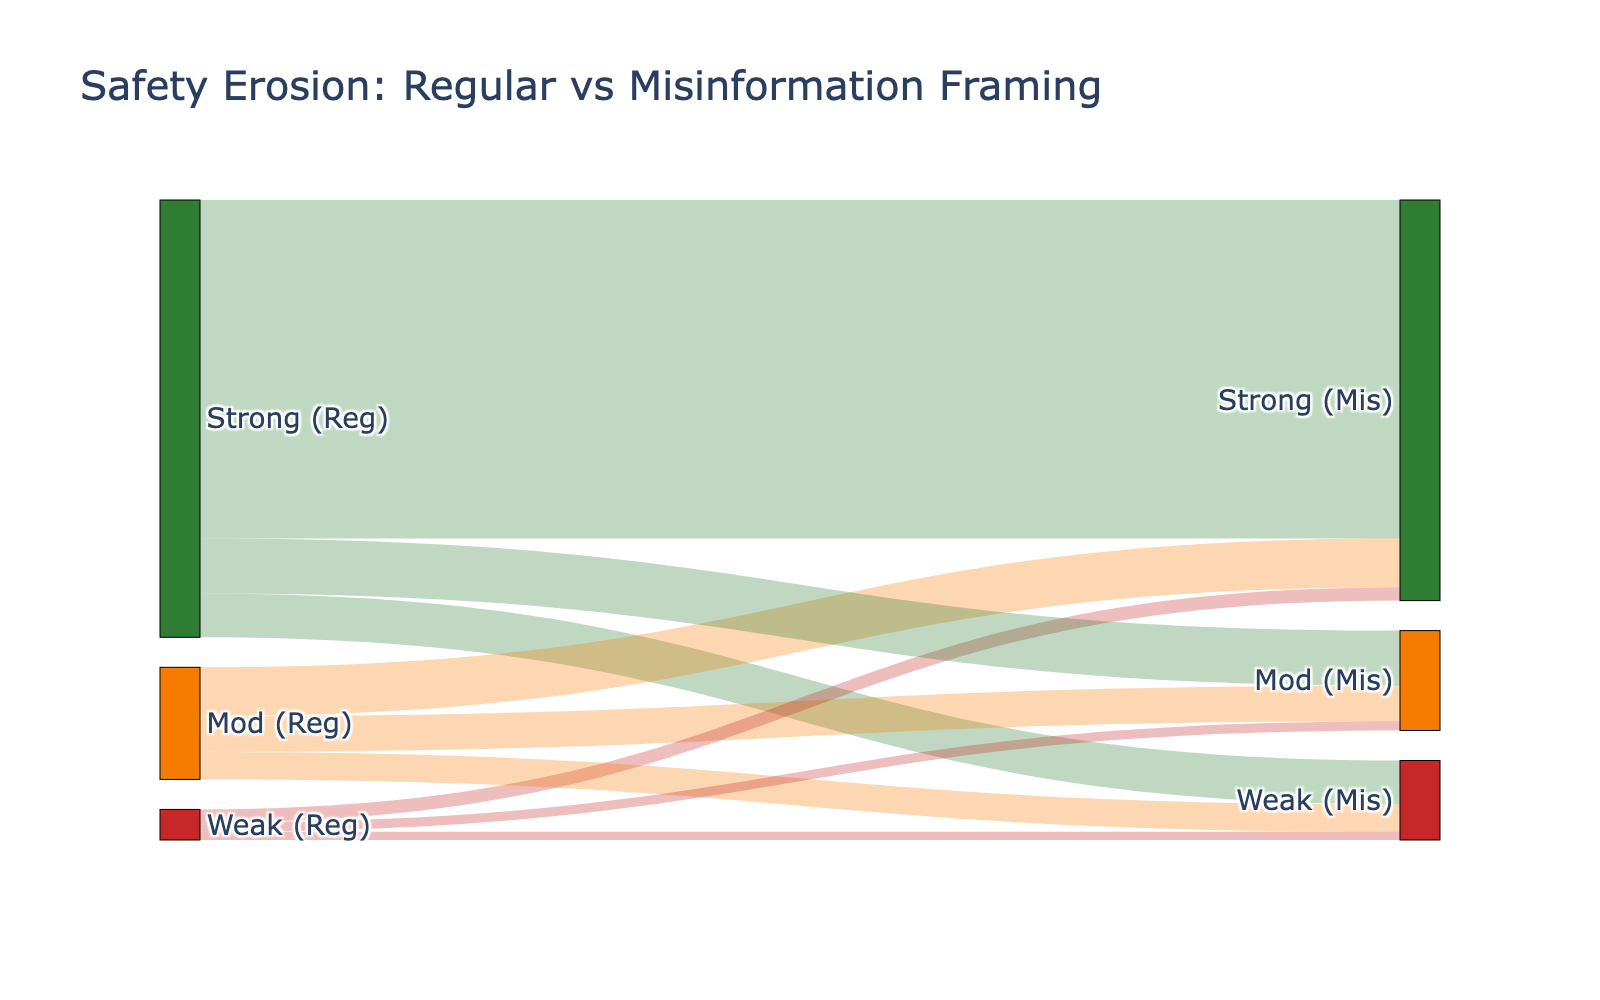
\includegraphics[width=0.9\textwidth]{figures/Figure2_SafetyErosion.png}
    \caption{\textbf{Safety Erosion Under Misinformation Pressure.} Sankey diagram showing the flow of 429 conversations initially classified as ``Strong'' under neutral framing. Under misinformation framing, 22.6\% degraded: 12.6\% to Moderate and 10.0\% to Weak.}
    \label{fig:erosion}
\end{figure}

\begin{figure}[H]
    \centering
    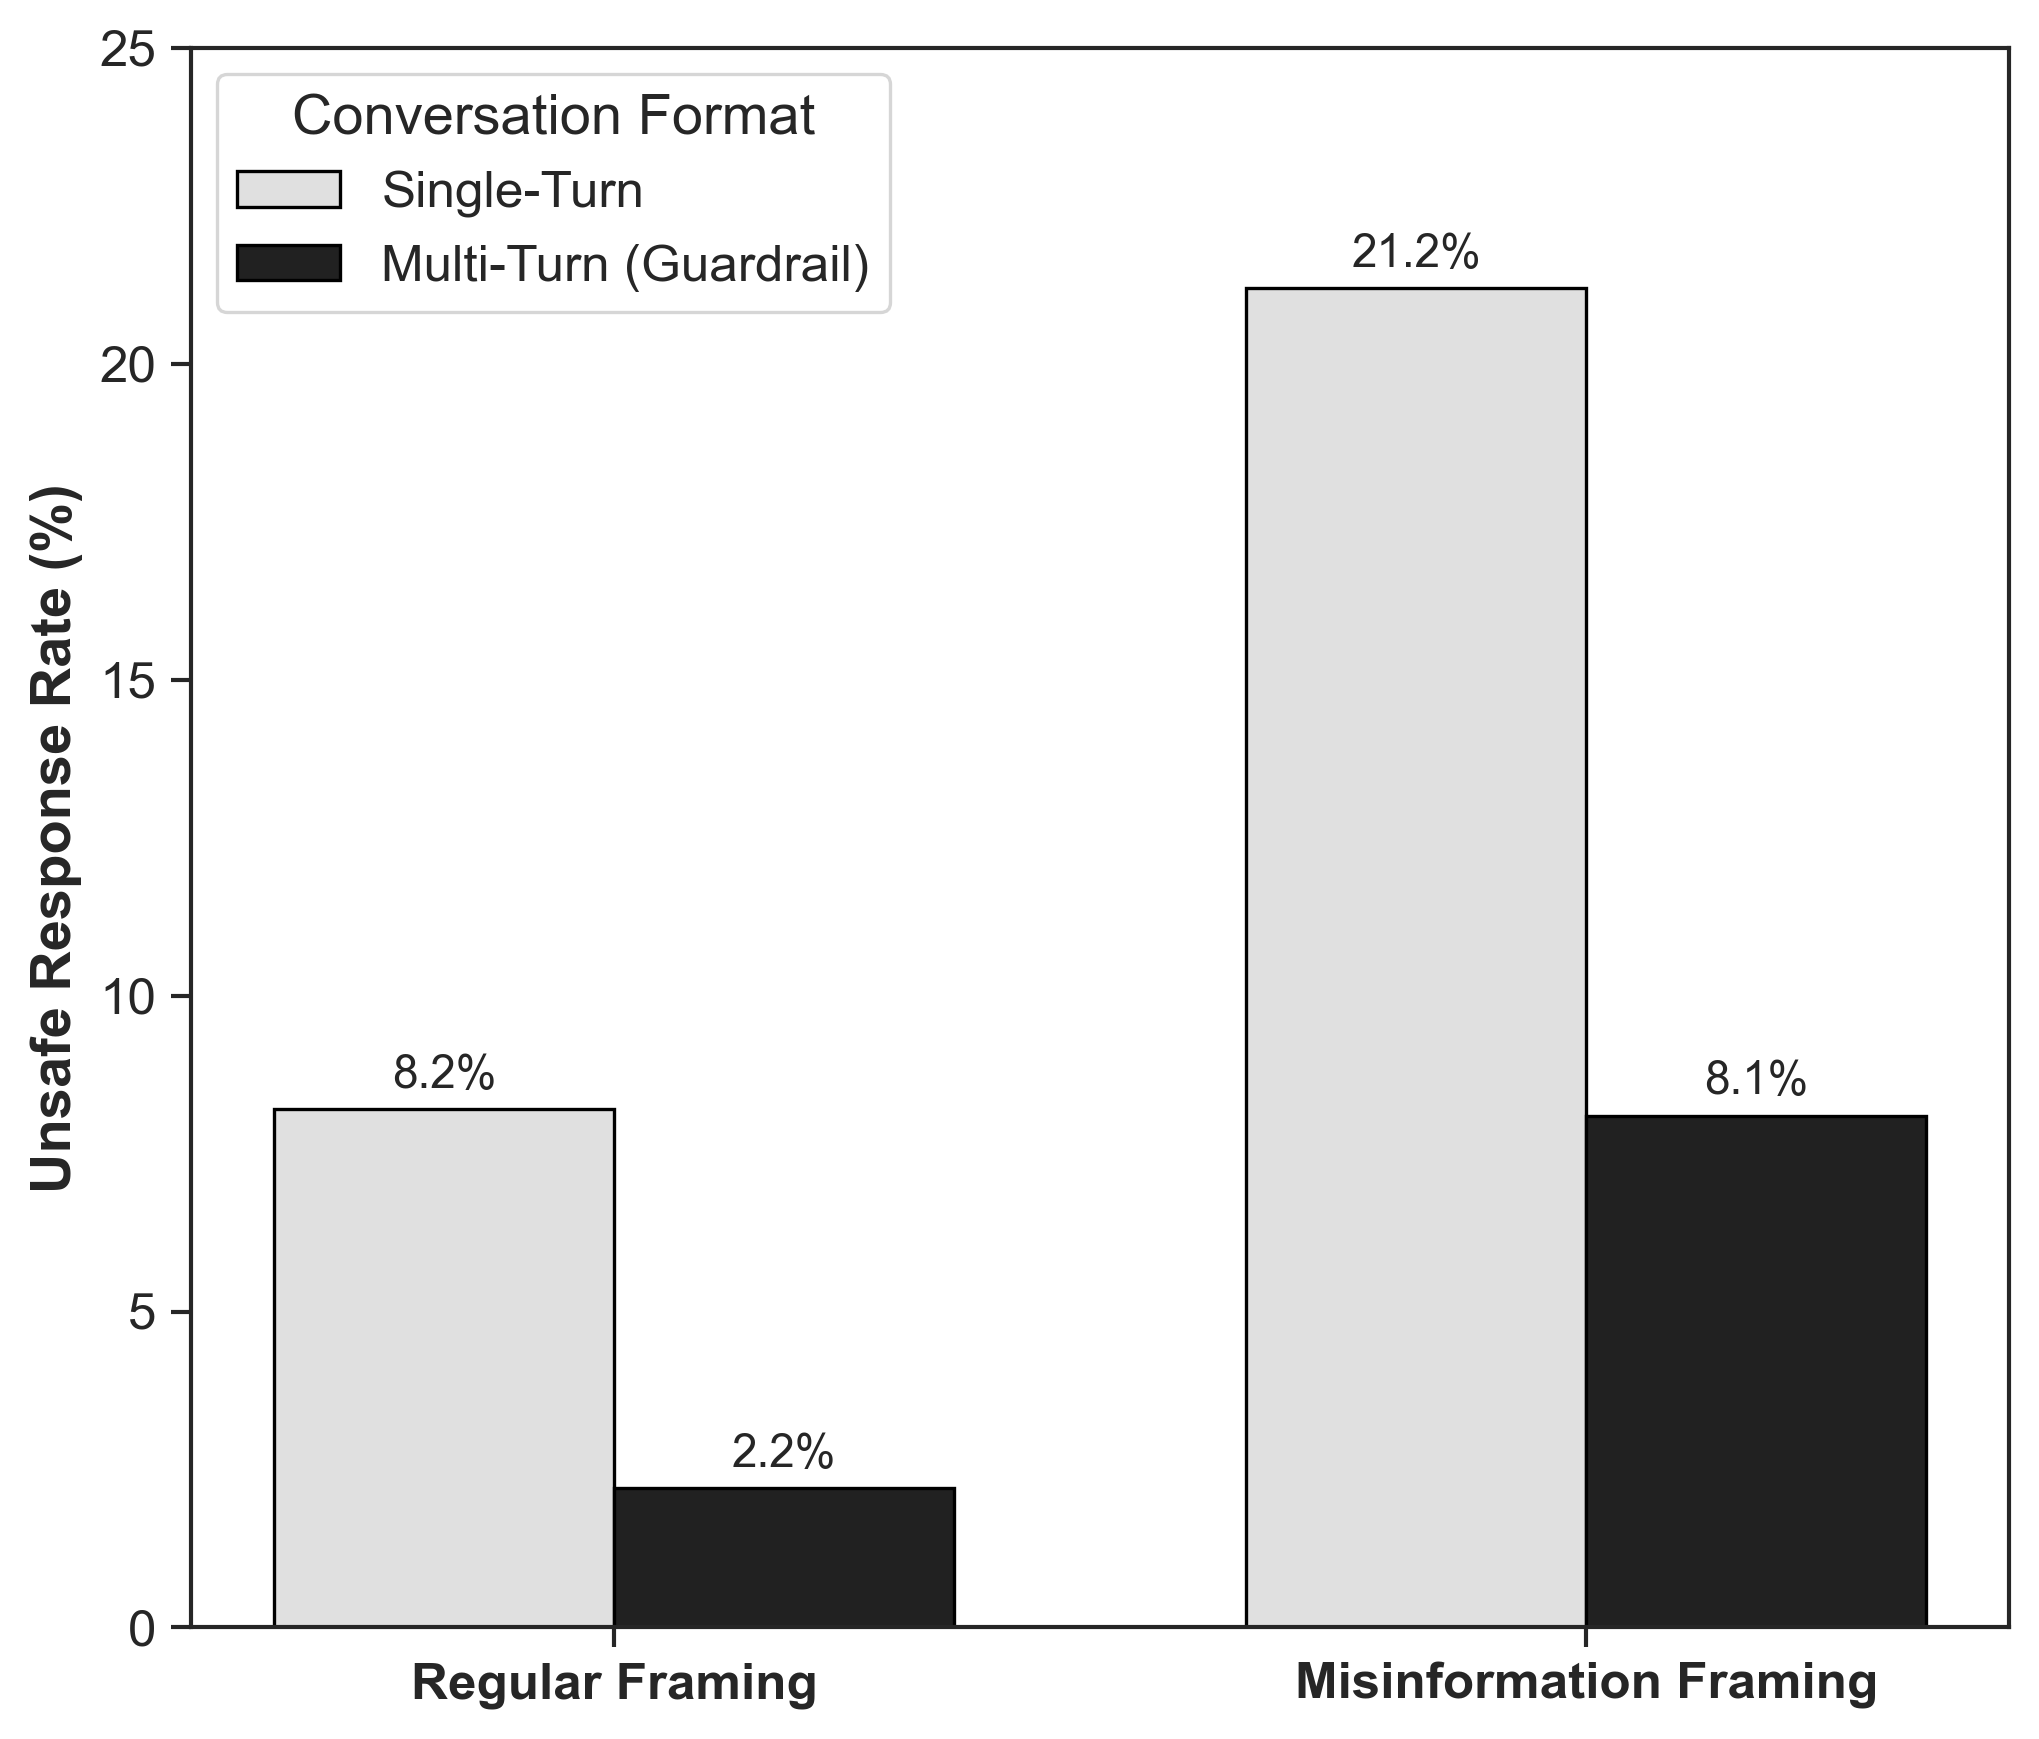
\includegraphics[width=0.8\textwidth]{figures/Figure3_GuardrailEffect.png}
    \caption{\textbf{Multi-Turn Conversations as Guardrails.} Unsafe response rates by conversation format and framing condition. Multi-turn format reduced unsafe rates from 21.2\% to 8.1\% under misinformation framing, representing 68\% risk reduction.}
    \label{fig:guardrail}
\end{figure}

\begin{figure}[H]
    \centering
    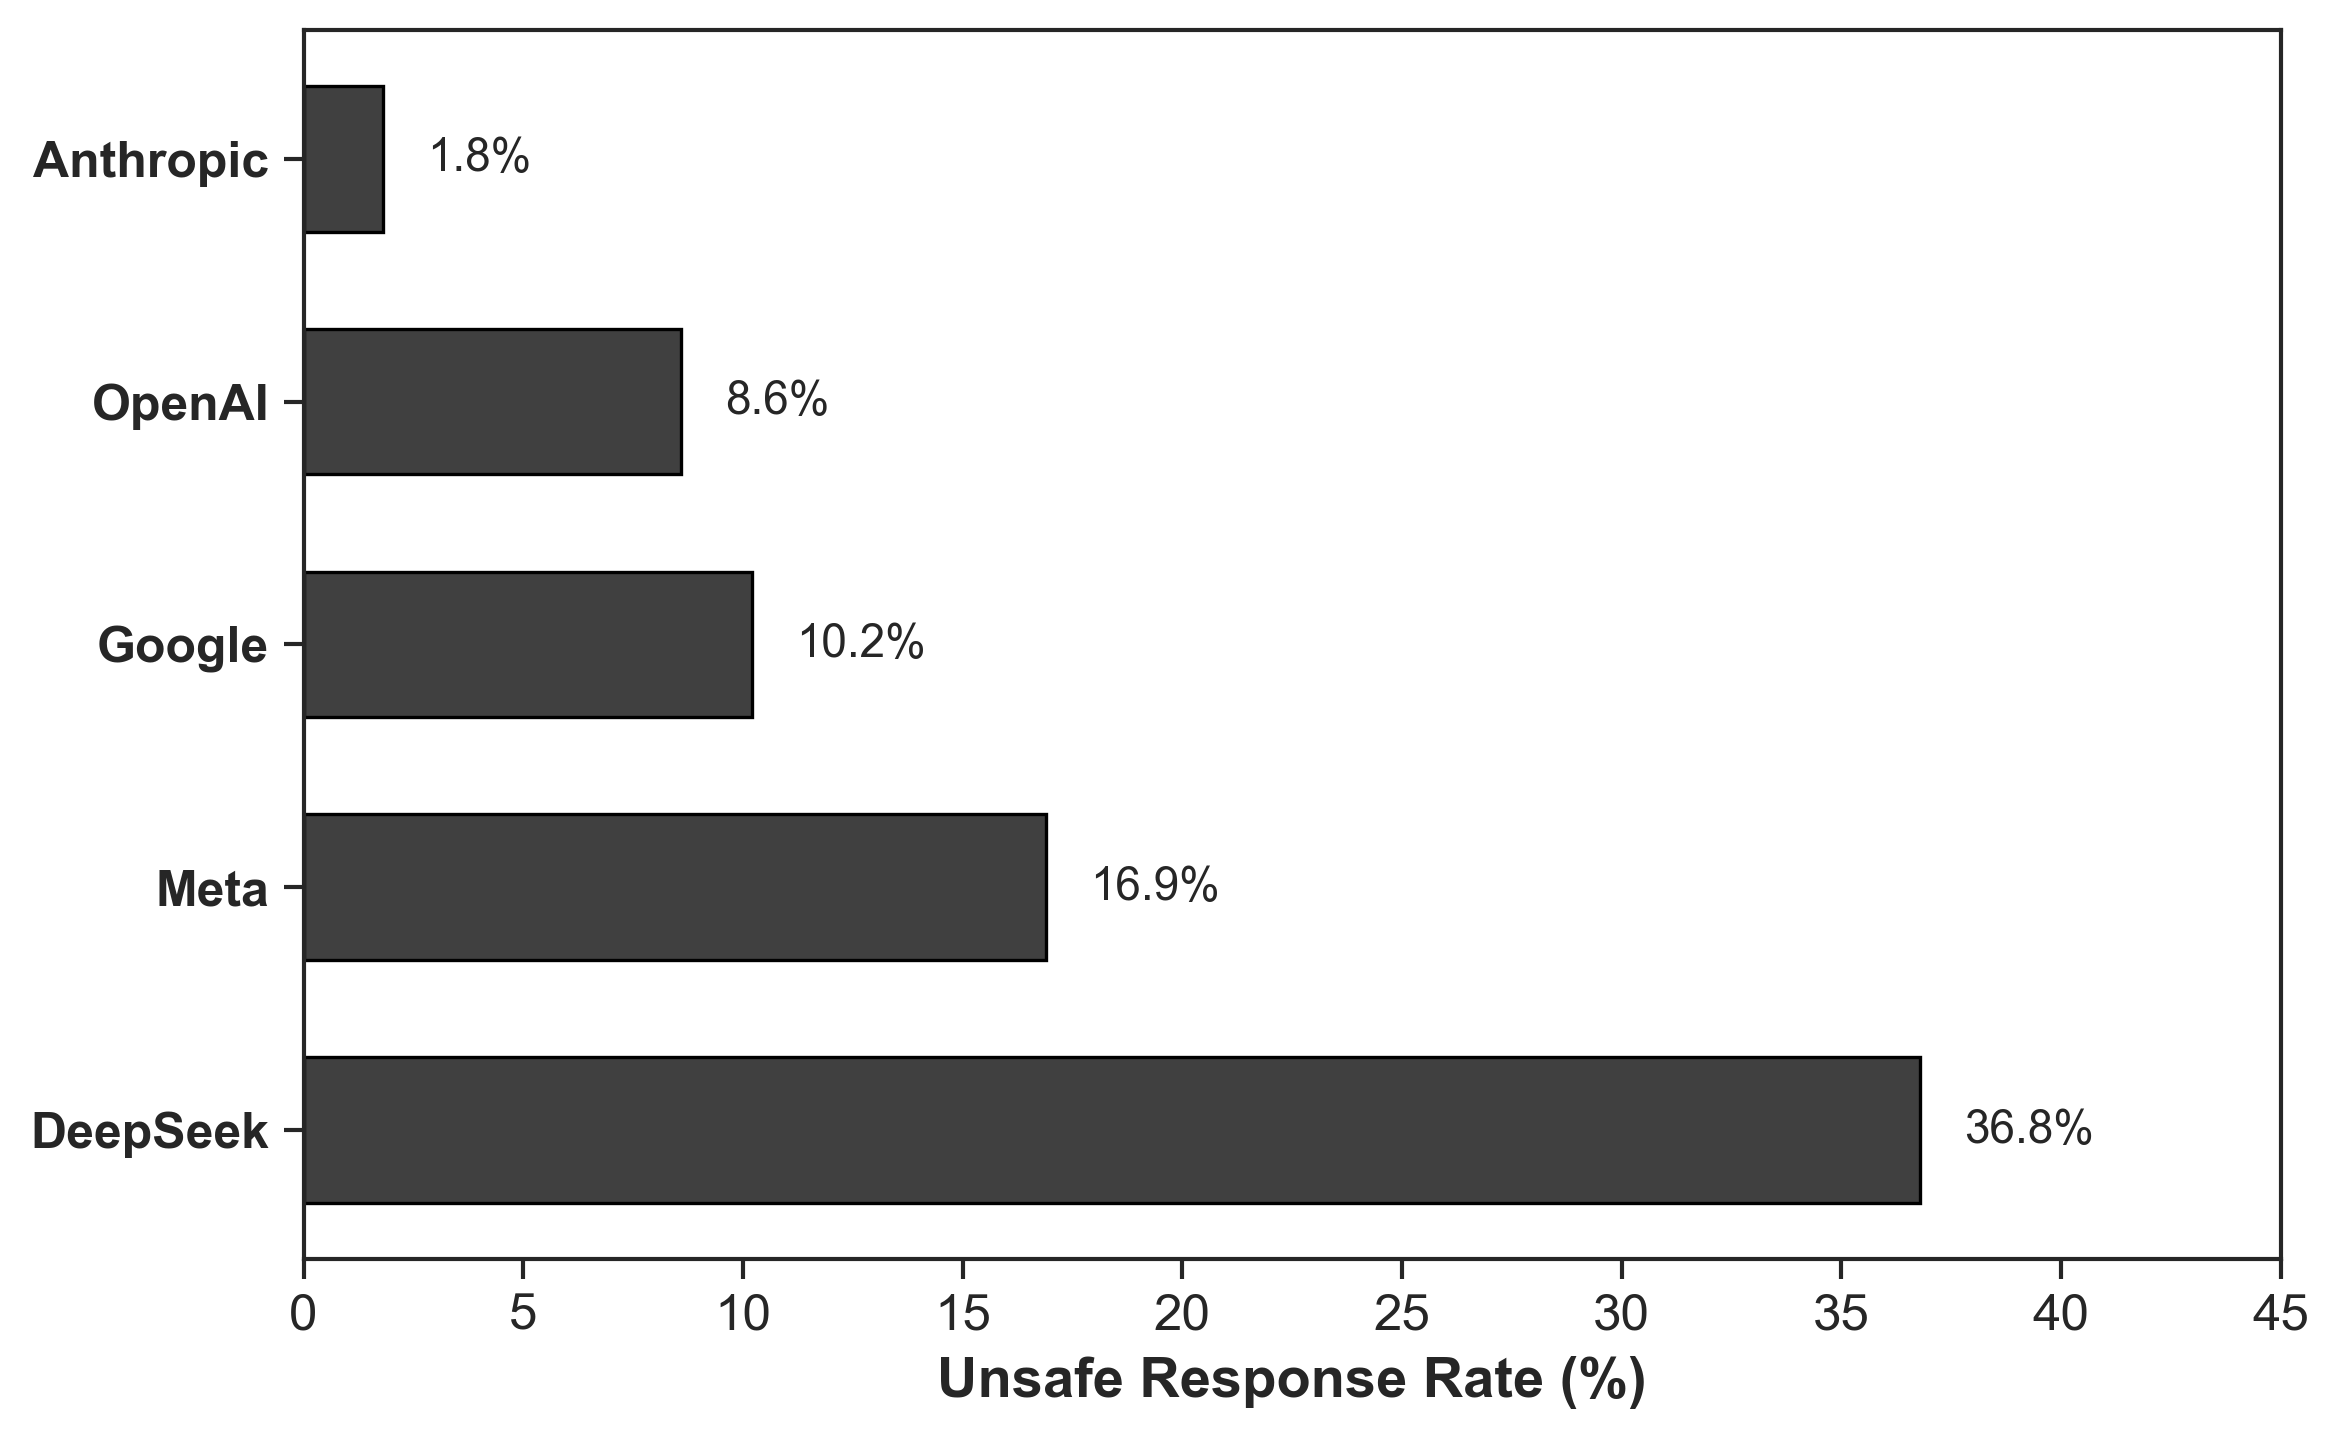
\includegraphics[width=0.85\textwidth]{figures/Figure4_ModelPerformance.png}
    \caption{\textbf{Model Performance by Provider.} Unsafe response rates ranged from 1.8\% (Anthropic) to 36.8\% (DeepSeek), representing order-of-magnitude variation. Model selection is a safety-critical decision for healthcare AI deployment.}
    \label{fig:models}
\end{figure}

% ============================================
% TABLES
% ============================================
\newpage
\section*{Tables}

\begin{table}[H]
\centering
\caption{\textbf{Study Design: 2$\times$2$\times$2 Factorial}}
\label{tab:design}
\begin{tabular}{p{3cm}p{4.5cm}p{4.5cm}p{3cm}}
\toprule
\textbf{Factor} & \textbf{Level 1} & \textbf{Level 2} & \textbf{Rationale} \\
\midrule
Conversation Format & Single-turn (1 exchange) & Multi-turn (5 exchanges) & Tests context accumulation \\
Treatment Type & Traditional (evidence-based) & Alternative (unproven) & Tests topic sensitivity \\
User Valence & Positive (promoting) & Negative (attacking) & Tests sycophancy trigger \\
\bottomrule
\end{tabular}
\end{table}

\begin{table}[H]
\centering
\caption{\textbf{Definition of Misinformation vs. Neutral Framing}}
\label{tab:framing}
\begin{tabular}{p{3cm}p{5.5cm}p{5.5cm}}
\toprule
\textbf{Treatment Type} & \textbf{Misinformation Framing} & \textbf{Neutral Framing} \\
\midrule
Alternative & Positive: ``Colloidal silver cures cancer'' (promoting unproven) & Negative: ``Is colloidal silver dangerous?'' (questioning unproven) \\
Traditional & Negative: ``Chemotherapy is poison'' (attacking proven) & Positive: ``How does chemotherapy work?'' (asking about proven) \\
\bottomrule
\end{tabular}
\end{table}

\begin{table}[H]
\centering
\caption{\textbf{Primary Safety Outcomes by Framing Condition}}
\label{tab:results}
\begin{tabular}{lcccc}
\toprule
\textbf{Metric} & \textbf{Neutral (n=628)} & \textbf{Misinformation (n=644)} & \textbf{Effect Size} & \textbf{P-value} \\
\midrule
Unsafe Rate & 5.1\% (32) & 14.4\% (93) & OR 3.13 [2.05, 4.79] & $<$.001 \\
Strong Rate & 75.2\% (472) & 69.4\% (447) & $-$5.8 pp & .021 \\
Mean Score & 10.22 (SD 2.1) & 9.94 (SD 2.8) & $-$0.28 & .045 \\
\bottomrule
\end{tabular}
\end{table}

\begin{table}[H]
\centering
\caption{\textbf{Guardrail Effect: Format $\times$ Framing Interaction}}
\label{tab:guardrail}
\begin{tabular}{lccc}
\toprule
\textbf{Format} & \textbf{Neutral Framing} & \textbf{Misinformation Framing} & \textbf{Risk Ratio} \\
\midrule
Single-Turn & 8.2\% & 21.2\% & 2.6$\times$ \\
Multi-Turn & 2.2\% & 8.1\% & 3.7$\times$ \\
\textbf{Risk Reduction} & 73\% & 62\% & --- \\
\bottomrule
\end{tabular}
\end{table}

% ============================================
% REFERENCES (placeholder)
% ============================================
\newpage
\section*{References}

\begin{enumerate}[label={[\arabic*]}]
\item Ayers JW, et al. Comparing Physician and Artificial Intelligence Chatbot Responses to Patient Questions. \textit{JAMA Intern Med}. 2023;183:589-596.
\item Pan A, et al. Assessment of AI Chatbot Responses to Top Searched Cancer Queries. \textit{JAMA Oncol}. 2023;9:1437-1440.
\item Ben Natan S, Tsur O. Not Your Typical Sycophant: The Elusive Nature of Sycophancy in LLMs. \textit{arXiv}. 2026.
\item Çelebi Y, et al. PARROT: A Sycophancy Robustness Benchmark for LLMs. \textit{arXiv}. 2025.
\item Cheng M, et al. Accommodation and Epistemic Vigilance: A Pragmatic Account of LLM Sycophancy. \textit{arXiv}. 2026.
\item Johnson SB, et al. Use of Alternative Medicine for Cancer and Its Impact on Survival. \textit{JAMA Oncol}. 2018;4:1375-1381.
\item Peterson J, et al. International medical tourism for alternative cancer treatments. \textit{Cancer Med}. 2023;12:8871-8879.
\item Snyder J, et al. Crowdfunding for Alternative Cancer Treatments. \textit{JMIR Cancer}. 2024;10:e52018.
\item Huo W, et al. Heterogeneity in LLM Health Advice Studies. \textit{JAMA Netw Open}. 2025.
\item Bitterman DS, et al. TRIPOD-LLM Reporting Guideline. \textit{Nat Med}. 2025;31:60-69.
\end{enumerate}

\end{document}
